To validate our design decisions, we used a two-pronged approach that consists
of both real-world data collection from live Tor users and simulations on our
software implementation.

\subsection{Data Collection}
\label{subsec:datacollection}

We deployed a data collection system to look for empirical temporal information
about lifetime and bandwidth consumption in Tor circuits. Our objective is to
have a deeper understanding of typical Tor usage and whether such usage can
benefit from our channel-based payment system. For example, these measurements
might capture some notion about the type and magnitude of potential premium
traffic. We classify the traffic type based on the service connection
port. Besides the classical ports 80 and 443 used for web traffic, we aggregate
data from some other families including the WHOIS
protocol~\cite{daigle2004whois} and RWHOIS~\cite{williamson1994referral} from
ports 43 and 4321, respectively. The complete list of families is constructed
from the reduced exit policies which we run on our relays. This measurement
methodology allows us to reason based on application specific traffic.

% We interested to know about the distribution lifetime of Tor circuits for each
% port we allow. We are also interested to picture how many cells those circuits
% handled through their lifetime with some level of granularity.

\subsubsection{Efforts to preserve users privacy}

To ensure ethical experimentation, we first contacted the Tor research safety
board~\cite{torsafety}. The feedback we received was subsequently used to refactor our data
collection process.

Data from multiple exit relays was collected, stripped of origin metadata, and
aggregate on a central server. The data collected from each relay is itself an
aggregation which we perform inside the relay's memory. The data collection is
probabilistic; only 30\% of the circuits processed by our relays were considered
in order to maintain plausible deniability on the clients' behalf. The
aggregation is done inside bins of configurable size for every different traffic
family we consider. Once we collected enough data from a single family, we dump
the information on the disk, clear the data, and resume a new session. The final
information dumped contains an aggregation of 1600 circuits over an unspecified
time frame that is implicitly determined by the rate of user activity. The
following data was considered:

\begin{itemize}
\item \textbf{Time Profile}: The number of cells in each time interval
  (configured to be 5 seconds) since the success of the DNS request. This
  information sums inbound and outbound cells, and is aggregated over circuits
  by addition.
\item \textbf{Total Counts}: The total amount of cells processed by a
  circuit. This information is aggregated by taking the mean of fixed-size
  nearest neighbor bins.
\end{itemize}

Crucially, we do not record information linked to any single particular user
flow on disk. The code used for the data collection will be made available for
audit online.

\subsubsection{Observations}

Our measurements successfully captured several important pieces of information
for the design and justification of moneTor. For example, one important task is
determine the number of potential users that could benefit from paid
traffic. From Figure~\ref{fig:stats_b}, we observe that $\approx 82\%$ of
circuits carrying only web traffic exchanged less than 1000 cells. While we
cannot deduce any statements about users, we can speak to the fraction of
circuits that may benefit from a payment channel in the Tor network, since
around $50\%$ of them do not carry data and less than $17\%$ of them carry at
least one web page. The remaining $18\%$ would appear to be better candidates
for moneTor.

It is also evident from Figure~\ref{fig:stats_a} that most of the traffic
usually happens within the first few tens of seconds, and that all types of
traffic we collected seems to follow the same rule. From that result, we believe
that the reliability of payment is critical within the first few seconds,
especially from a relay viewpoint. Our payment channels should ideally be
established and ready before the user begins to use the circuit which is made
possible by our design decision to integrate into Tor's preemptive circuit build
strategy.

%% In another area of research, it may be interesting to point out that since %
%$\approx 50\%$ of users do not carry data after their DNS request, some %
%adversary doing end-to-end correlation may prefer to use active attacks over %
%passive correlation to capture more identities.

\begin{figure*} \centering
	\begin{subfigure}[t]{0.32\textwidth} \centering
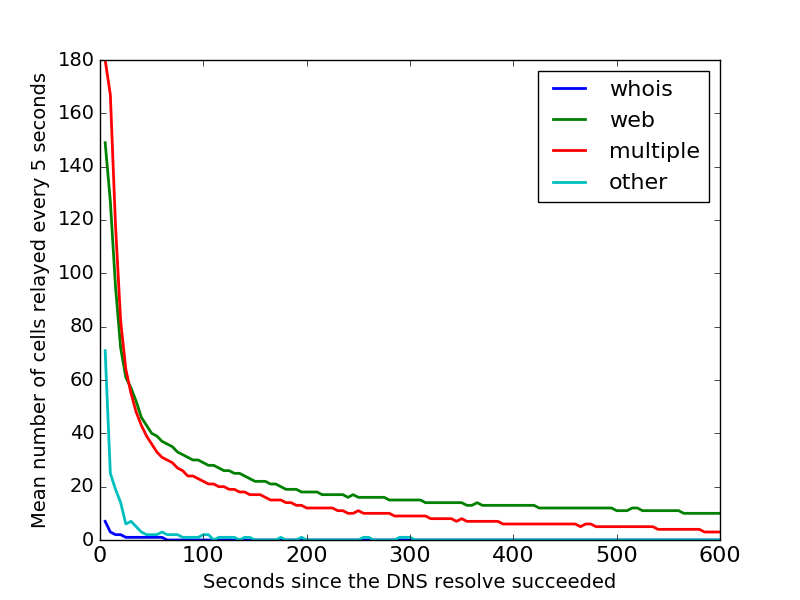
\includegraphics[scale=0.3]{images/exitmeasurement.png}
		\label{fig:stats_a}
		\caption{Time Profile}
	\end{subfigure}
	\begin{subfigure}[t]{0.32\textwidth} \centering
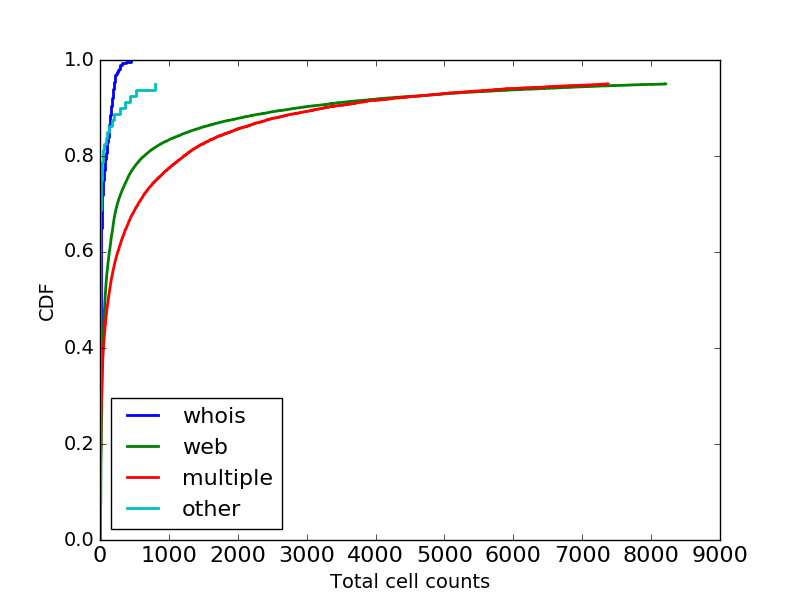
\includegraphics[scale=0.3]{images/totcellcountscdf.png}
		\label{fig:stats_b}
		\caption{Total Counts}
	\end{subfigure}
	\label{fig:measurements}
	\caption{Tor Measurements}
\end{figure*}

\section{Simulated Validation}

Having established the empirical context for a channel payment scheme, we
validated our technical design via experiments performed on a proof-of-concept
software implementation within the native Tor codebase.

\subsection{Prototype}

A substantial contribution of the research is embedded within our implementation
of the moneTor framework. The modifications, applied to Tor release version
0.3.2.10, cover approximately fifteen thousand added lines of code across Tor's
core C software. We emphasize that the implementation is not a fully functional
prototype and is optimized solely for our experiments. Most notably, we
simulated crytographic operations in the nanopayment creation and close
procedures using cpu delays. These delays were tuned to conservatively reflect
real measurments in background work~\cite{green2017bolt}.\footnote{Extracted
  values are conservative in the sense that our zero-knowledge proofs require
  proving only a subset of the statements required in each corresponding Bolt
  zero-knowledge proof.}  In spirit, the partial prototype serves the following
purposes in our study.

\begin{enumerate}
\item A proof-of-concept implementation covering nuances not explicitly
  covered in the protocol designs. In effect, we would like to show that there
  are no unexpected and prohibitive practical conflicts with the existing Tor
  design.
\item A platform to study the feasibility of premium circuit
  prioritization from a networking perspective.
\item A platform to obtain a rough factor-of-two approximation for all
  bandwidth, computation, and memory requirements of the system, both globally
  and at individual nodes.
\end{enumerate}

The first design purpose is clearly qualitative and we briefly note that we did
not discover any insurmountable logical flaws in the design. To analyze the
networking dynamics and resource consumption, we studied our implementations
through the following proceeding experiments.

\subsection{Methodology}
\label{subsec:methodology}

Experiments were conducted using the Tor shadow simulator
tool~\cite{jansen2011shadow}.
%Shadow is a discrete event networking simulator
%that allows real, unmodified applications to run within a virtual network. Its
%primary advantage is the ability to emulate native application code. Originally
%built for Tor, Shadow faithfully mimics the real Tor network conditions
%including bandwidth and latency while allowing greater scale and network
%accuracy than alternative test beds.
We approach the problem at multiple scales ranging between small (50 relays, 200
clients), medium (100 relays, 400 clients), and large (200 relays, 800
clients). Experiments ran for 1.5 hours of virtual time allowing for 30 minutes
of bootstrapping and one hour of simulated steady state traffic. Simulated
traffic features 16\% \emph{bulk} clients who continuously download 5 MiB files
and 84\% \emph{web} clients who periodically download 2 MiB
files,\footnote{While 5 MiB bulk files are a common standard in Tor
  benchmarking~\cite{portal2018tormetrics}, 2 MiB web files reflect the
  approximate size of modern web pages~\cite{team2018httparchive}} pausing
between 1 and 60 seconds inbetween. In all cases, the number and behavior of
clients were chosen to satisfy (A) realistic congestion rates measured by a
transfer timeout percentage around 4\%~\cite{portal2018tormetrics} and a historical
bulk/web global traffic ratio of about 50\%~\cite{chaabane2010digging,
  mccoy2008shining}. Importantly, it should be noted that neither the scale of
our experiments nor the precise configuration of client nodes are intended to be
precise replicas of real-world conditions. Tor networking is itself a complex
area of research and we are content to adopt the simplest model that will
highlight the relatively crude networking needs of our payment scheme.

\subsection{Experiments}
\label{subsec:experiments}
Our experiments are separated into three groups each capturing a separate
characteristic of the scheme.

\subsubsection{Global Overhead}

First, we attempt to show the total cost the moneTor scheme in terms of total
network throughput. To highlight worst-case performance, we configured a medium
scale experiment consisting of 100\% of premium clients and compare to a
baseline trial with 0\% premium clients. No actual traffic priority is
conferred. Since our algorithms makes use of some concurrent crytpographic
operations, we are concerned with the number of CPU cores available to most
relays. This information is not publically available. As a result, we performed
provide two trials with moneTor: one where we assume all nodes are running on
multi-core hardware and one in which all nodes are running on single-core
hardware. The results are summarized in Figure~\ref{fig:overhead_throughput} and
Figure~\ref{fig:overhead_ttlastbyte}.

\begin{figure*} \centering
	\begin{subfigure}[t]{0.32\textwidth} \centering
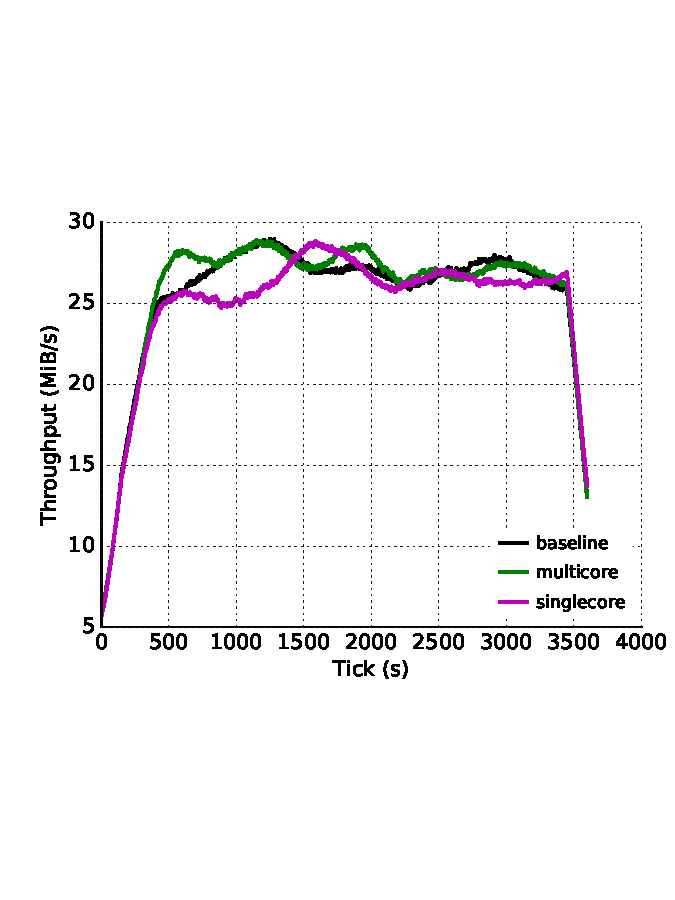
\includegraphics[trim={0 3cm 0 3cm}, clip, width=1.0\textwidth]{images/overhead_throughput.pdf}
		\label{fig:stats_a}
		\caption{Throughput Overhead}
	\end{subfigure}
	\begin{subfigure}[t]{0.32\textwidth} \centering
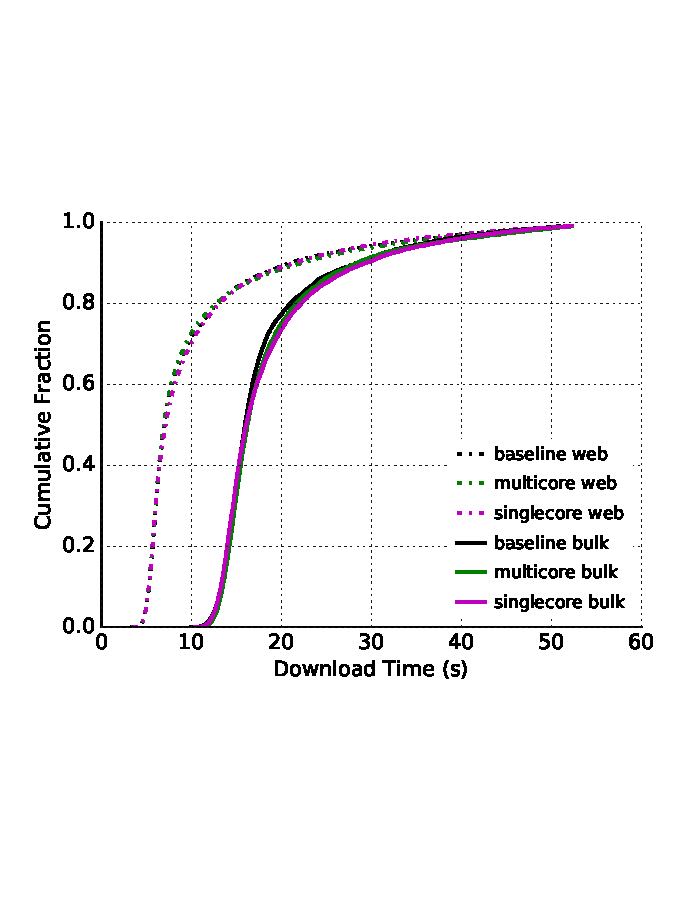
\includegraphics[trim={0 3cm 0 3cm}, clip, width=1.0\textwidth]{images/overhead_downloadtime.pdf}
		\label{fig:stats_b}
		\caption{Download Time Overhead}
	\end{subfigure}
%	\begin{subfigure}[t]{0.32\textwidth} \centering
%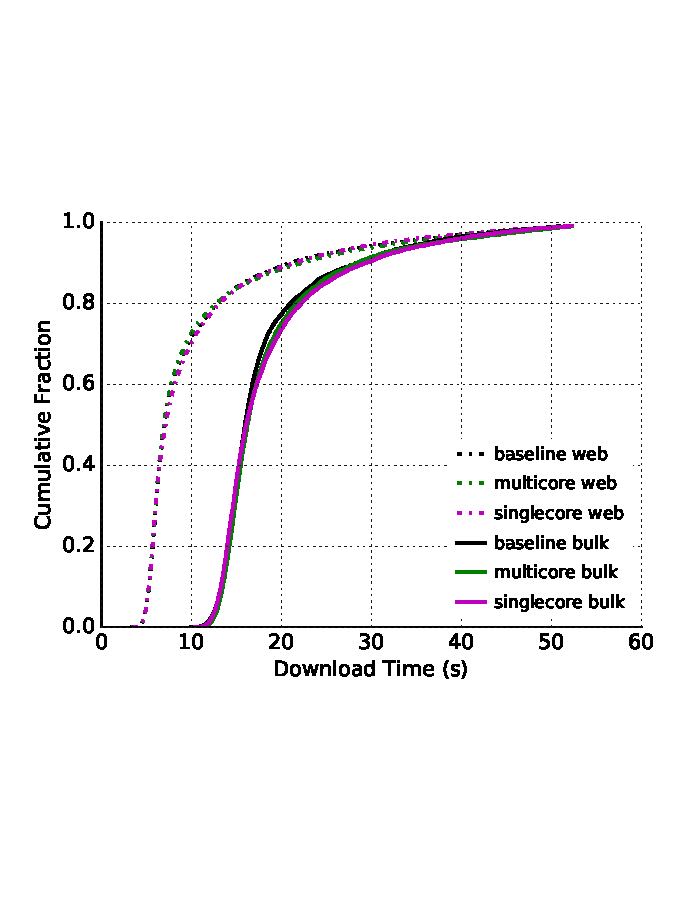
\includegraphics[trim={0 3cm 0 3cm}, clip, width=1.0\textwidth]{images/overhead_downloadtime.pdf}
%		\label{fig:stats_c}
%		\caption{Time Stdevs}
%	\end{subfigure}
	\label{fig:measurements}
	\caption{moneTor Overhead}
\end{figure*}

Our findings indicate that even the worst case scenario our system incurs
statistically negligible overhead at these scales. This result is explained by
raw values shown in Table~\ref{tab:overhead}, which indicates that less than
0.4\% of the network traffic is attributable to moneTor payment messages.

\begin{table}
  \caption[Overhead Throughput Total]{\textbf{Overhead Throughput Total} Total
    transferred application traffic over the duration of the over head trials
    compared to total transferred payment traffic.}
  \begin{center}
    \begin{tabular}{ c c c }
      & Throughput (GiB) & Payment Traffic (GiB) \\ \hline
      Baseline & 128.4 & 0.000 \\
      Multi-Core & 129.1 & 0.449 \\
      Single-Core & 127.6 & 0.396
    \end{tabular}
  \end{center}
  \label{tab:overhead}
\end{table}

\subsubsection{Payment Latency}

Given results from \autoref{chap:empirical}, we surmise that payment
latency is a crucial factor in servicing our front-loaded clients. To this end,
we measure the distribution of completion times for various steps in the
protocol. The results shown here are collected from a large experiment featuring
50\% premium clients. To highlight the effects of native latency in the Tor
network, we show payments split across each relay role of guard, middle, and
exit.

Recall that moneTor makes use of high-overhead, low-marginal cost payment
channels. The bulk of the cost in our scheme lies in the conduction of the
nanopayment channel \emph{establish} and \emph{close} protocols as shown in
Figure~\ref{fig:payments_establish} and Figure~\ref{fig:payments_close}. Notice
that close operations are about twice as time consuming as establish operations
reflecting the need for the relay to close his half of the nanopayment channel
before the client can complete hers.

\begin{figure*} \centering
	\begin{subfigure}[t]{0.32\textwidth} \centering
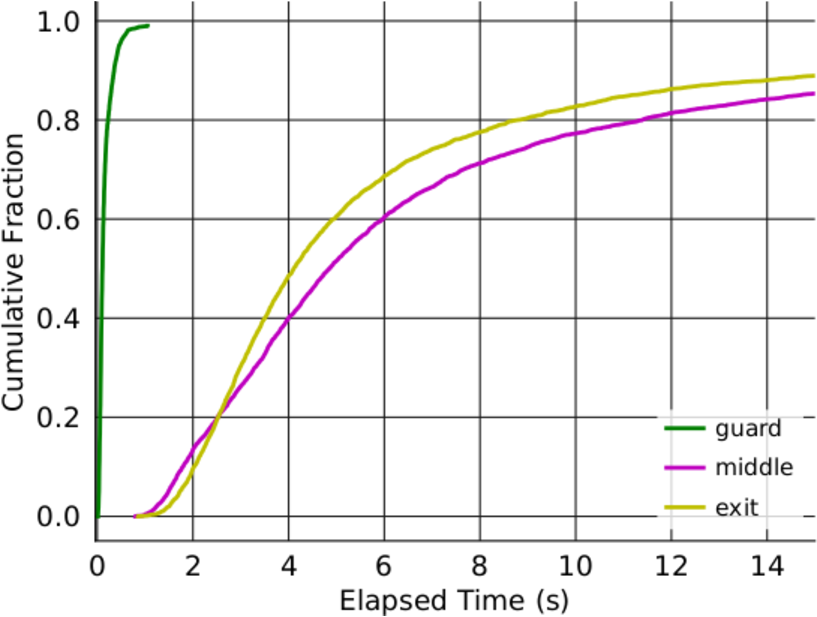
\includegraphics[trim={0 3cm 0 3cm}, clip, width=1.0\textwidth]{images/payment_establish.pdf}
		\label{fig:stats_a}
		\caption{Time to Establish}
	\end{subfigure}
	\begin{subfigure}[t]{0.32\textwidth} \centering
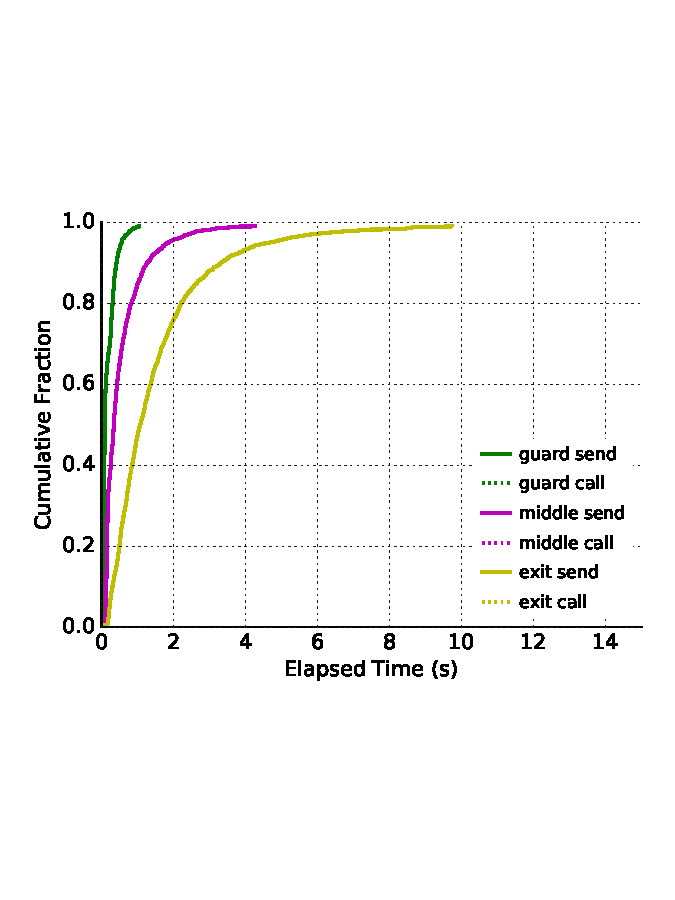
\includegraphics[trim={0 3cm 0 3cm}, clip, width=1.0\textwidth]{images/payment_pay.pdf}
		\label{fig:stats_b}
		\caption{Time to First Payment}
	\end{subfigure}
	\begin{subfigure}[t]{0.32\textwidth} \centering
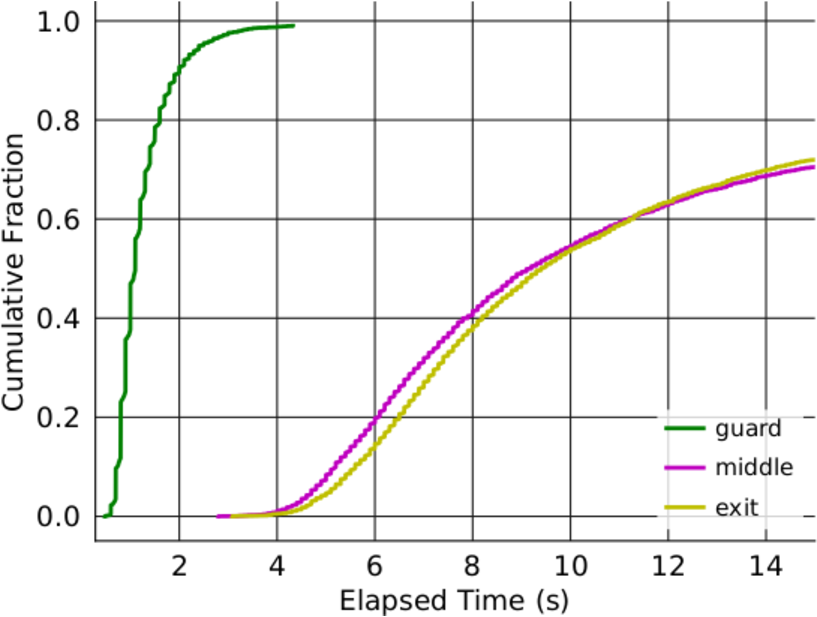
\includegraphics[trim={0 3cm 0 3cm}, clip, width=1.0\textwidth]{images/payment_close.pdf}
		\label{fig:stats_c}
		\caption{Time to Close}
	\end{subfigure}
	\label{fig:measurements}
	\caption{Protocol Execution Time}
\end{figure*}


Figure~\ref{fig:payments_pay} illustrates time to first payments, our most
revealing latency metric. The figure superimposes the time to first payment as
measured from when the client would first like to send a payment (call) and the
time when she actual does send the payment (send). The first measure includes
the overhead in channel establishment when we do not have available preemptive
channels. The second measure is essentially equivalent to one round trip time to
each of the relays and represents a theoretical best-case bound for any payment
system. Note from the juxtaposition of these two measures that our effective
time to first payment (call) is generally much faster than the raw time to
establish period, indicating the effectiveness of preemptive channel building.

In all protocol phases, we observe that latency for guard relays are negligible
in comparison to the middle and exit relays, further validating our design
decision to implement special directly paid guard channels.

\subsubsection{Network Priority}
\label{sec:priority_exp}

Our final set of experiments studies the success of our scheme in delivering
prioritized traffic for premium users. To perform this analysis, we prepared
sets of three small experiments with varying modifier priorities
$\alpha \in \{0, 0.25, 0.5\}$, where $\alpha = 0$ represents the baseline
control. Our first set of experiments assuming 50\% of premium users is shown in
Figure~\ref{fig:modifier_pr50}. From this illustration, is it evident that
premium users enjoy an advantage in internet speed compared to nonpremium users
and that this advantage is more pronounced with the higher priority
modifier. Moreover, the evenly split premium and nonpremium performance
``averages out'' to approximately mirror the baseline experiment, indicating
little loss in overall network performance.

We modified our experiment to study an environment comprised of only 25\%
premium users who, according to Equation~\ref{eq:flow}, should enjoy even
greater benefit. Figure~\ref{fig:modifier_pr25} shows that this is indeed the
result. Slower users in the lower 20th percentile of download speeds enjoyed
$\approx 200\%$ improvements in download speeds relative to nonpremium users ---
likely enough to induce some amount of monetary exchange.

\begin{figure*} \centering
  \begin{subfigure}[t]{0.32\textwidth} \centering
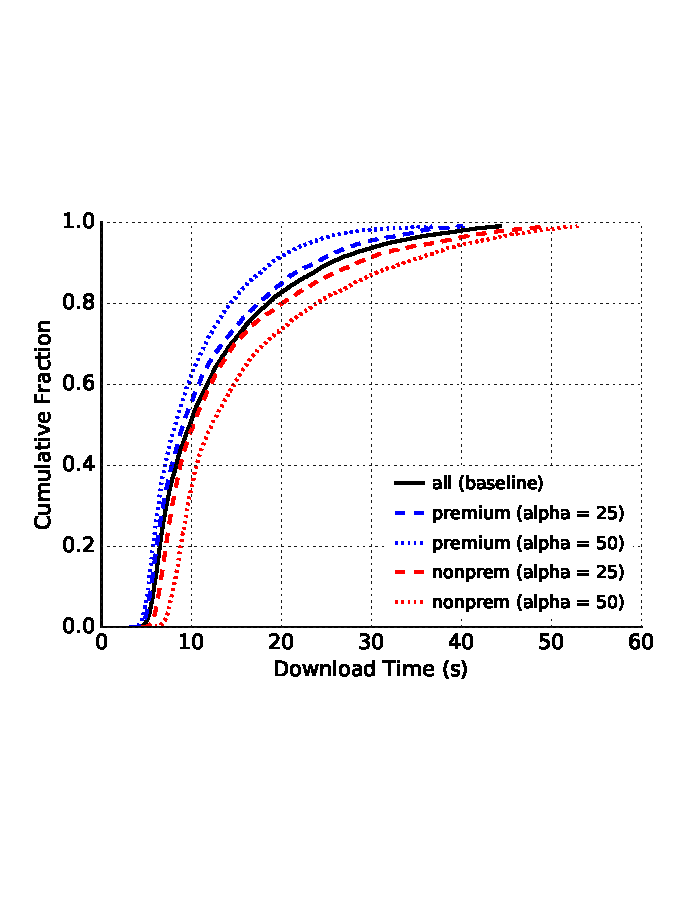
\includegraphics[trim={0 3cm 0 3cm}, clip, width=1.0\textwidth]{images/modifier_pr50_web.pdf}
		\label{fig:stats_a}
		\caption{Prioritized Web (50\% Premium)}
	\end{subfigure}
	\begin{subfigure}[t]{0.32\textwidth} \centering
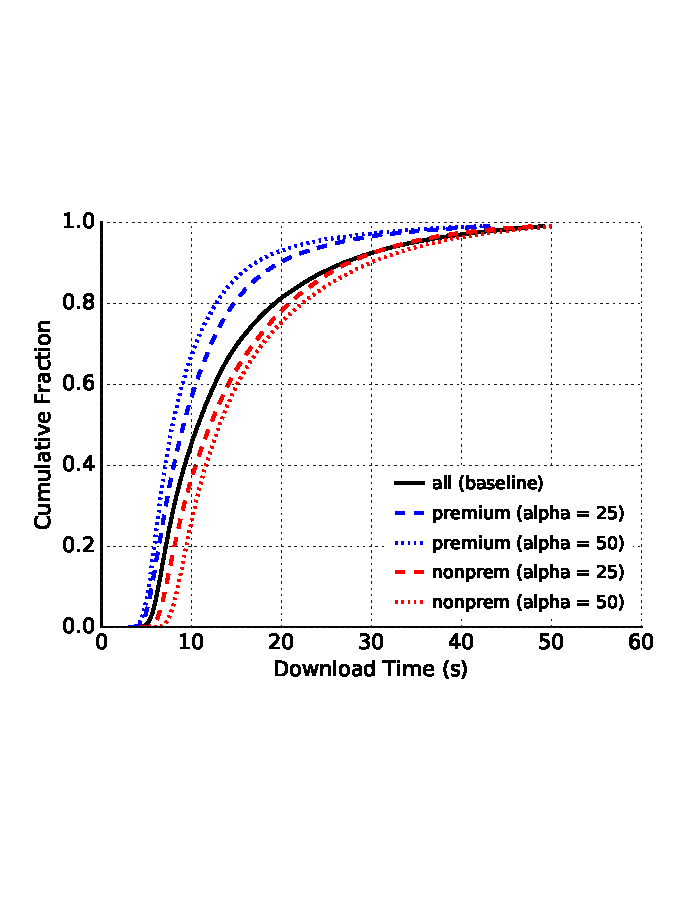
\includegraphics[trim={0 3cm 0 3cm}, clip, width=1.0\textwidth]{images/modifier_pr25_web.pdf}
		\label{fig:stats_b}
		\caption{Prioritized Bulk (50\% Premium)}
	\end{subfigure}
	\begin{subfigure}[t]{0.32\textwidth} \centering
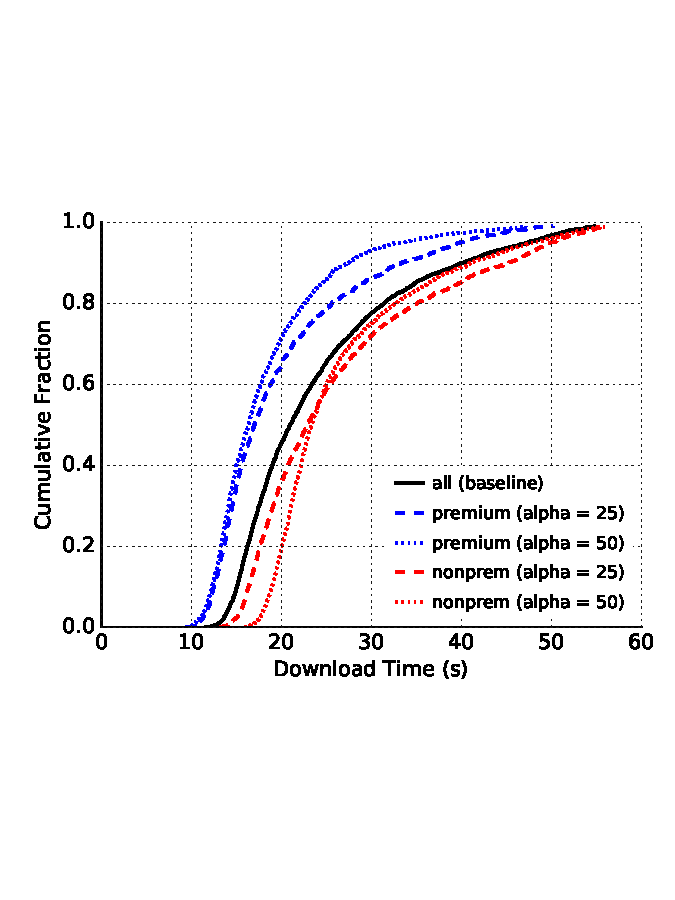
\includegraphics[trim={0 3cm 0 3cm}, clip, width=1.0\textwidth]{images/modifier_pr25_bulk.pdf}
		\label{fig:stats_c}
		\caption{Prioritized Web (25\% Premium)}
	\end{subfigure}
	\label{fig:measurements}
	\caption{Prioritization Benefit}
\end{figure*}

Finally, we note that while we performed similar experiments for $\alpha = 0.75$
we observed that network performance as a whole suffered dramatically. The crude
numbers are quantified in Table~\ref{tab:modifier}. At more reasonable
prioritization levels, however, the performance loss from network imbalance is
statistically negligible at this scale.

\begin{table}
  \caption[Prioritized Throughput]{\textbf{Prioritized Throughput} Tabulate total
    number of successful file transfers and timeout errors across varying levels
    of prioritization}
  \begin{center}
    \begin{tabular}{ c c c c}
      & Throughput & Timeouts & Timeout \\
      & (GiB) & (Web) & (Bulk) \\ \hline
      $\alpha = 0.00$ & 46.6 & 115 & 354 \\ \hline
      $\alpha = 0.25,\ pr\% = 50$ & 46.2 & 206 & 404 \\
      $\alpha = 0.25,\ pr\% = 25$ & 46.0 & 231 & 459 \\ \hline
      $\alpha = 0.50,\ pr\% = 50$ & 46.4 & 233 & 356 \\
      $\alpha = 0.50,\ pr\% = 25$ & 44.9 & 381 & 513 \\ \hline
      $\alpha = 0.75,\ pr\% = 50$ & 41.55 & 902 & 571 \\
      $\alpha = 0.75,\ pr\% = 25$ & 36.1 & 1403 & 740 \\

    \end{tabular}
  \end{center}
  \label{tab:modifier}
\end{table}
